\documentclass[tikz]{standalone}
\begin{document}
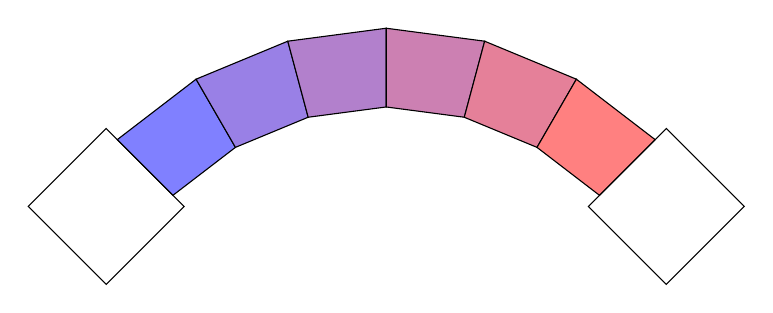
\begin{tikzpicture}
\newcommand*\myAng   {7.5}
\newcommand*\myArches{5} % starting with 0
\coordinate (@);
\foreach[evaluate={\c=\i/\myArches*100;}] \i in {0,...,\myArches}
  \draw[rotate=-(\i-(\myArches-1)/2)*2*\myAng+\myAng, fill=red!\c!blue!50]
    (@) -- +(90+\myAng:1)
        -- +([shift=(90-\myAng:1)]right:1)
        -- +(right:1) coordinate (@)
        -- cycle;

\draw[rotate= (\myArches+1)*\myAng]          (0, -0.2)     rectangle +(-1.4, 1.4);
\draw[rotate=-(\myArches+1)*\myAng] ([shift={(0, -0.2)}]@) rectangle +( 1.4, 1.4);
\end{tikzpicture}
\end{document}